%------------------------------début entêtes-----------------------------------------
\pagestyle{fancy}

\renewcommand{\footrulewidth}{1pt}

\fancyhead[L]{\footnotesize \rightmark}
\fancyhead[C]{\thepage}
\fancyhead[R]{Acronymes}

\fancyfoot[L]{Ny Hoavy Nomena}
\fancyfoot[C]{\thepage}
\fancyfoot[R]{Annotation automatique d'images}
%Enlever le mot chapitre
%\titleformat{\chapter}[hang]{\bf\huge}{\thechapter}{2pc}{}
%\titleformat{\chapter}[hang]{\bf\huge}{Partie \thechapter : }{2pc}{}
%\def\chaptername{Partie}
%\def\chapternum{none}

%------------------------------fin entêtes-------------------------------------------

\chapter*{Les RNA pour l'apprentissage profond} \label{rna}

Cette section est dédiée à une présentation générale des Réseaux de Neurones Artificiels (RNA) et de l'apprentissage profond \cite{deepweb}. Nous ne présentons que les méthodes les plus utilisées dans  les travaux étudiés.\\
\smallskip

\qquad Un réseau de neurones artificiels est un modèle connexionniste qui utilise les informations numériques pour effectuer des calculs analogues à ceux d'un neurone. Les modèles neuronaux imitent la biologie et reproduisent les mécanismes de base naturels.\\
	Les réseaux sont constitués de couches successives constituées de neurones. Ces couches sont interconnectées à partir de ces neurones : les neurones de la l-ème couche, qui sont activés, envoient des données aux neurones de la couche suivante par des connections pondérées qui à leur tour calculent leur valeur d'activation ou sortie et la diffusent.\\
	Pour une explication plus formelle, nous allons voir l'architecture générale d'un RNA et établir les différentes expressions des traitements effectués par le réseau.\\
En général, un réseau de neurones est composé d'une couche d'entrée, d'une ou plusieurs couches cachées et d'une couche de sortie.

\begin{figure}[h]
	\begin{center}
		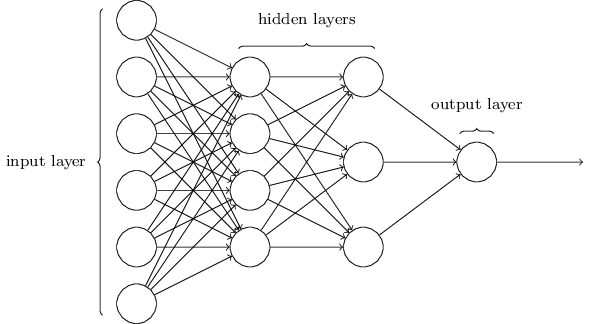
\includegraphics[width=0.7\textwidth]{rna}
		\caption{Architecture générale d'un réseau de neurones artificiels}
	\end{center}
\end{figure}
\smallskip

La couche d'entrée est composée de neurones qui correspondent aux caractéristiques des données d'entrée représentées par une grille multidimensionnelle (par exemple la matrice de pixels de l'image). La couche de sortie représente les résultats de la tâche assignée au réseau. Par exemple pour une classification de 1000 classes, les 1000 neurones de la couche de sortie représentent la probabilité pour chaque classe.\\
\smallskip
\textbf{Propagation directe:}\\
La propagation directe est le traitement des données d'entrée du réseau jusqu'au calcul des sorties. Ainsi le traitement des données d'entrée se propage de couche en couche. Pour chaque neurone d'une couche l, les entrées (activations des neurones voisins) issus des connexions de ses neurones voisins sont sommées par rapport au poids de chaque connexion pour calculer sa valeur d'activation à partir d'une fonction non-linéaire appelée : fonction d'activation.
Pour le $j$-ème neurone du $l$-ème couche, on définie sa valeur d'activation $a^l$ par rapport à aux sorties de la $(l-1)$-ème couche des neurones voisins \footnote{Il est à préciser que les neurones d'une couche donnée ne sont pas toujours connectés à tous les neurones de la couche adjacente. Les réseaux de neurones convolutifs utilisent d'autres formes de connection plus complexe. Si c'est le cas, on parle de couches interconnectées}:
\begin{eqnarray} a^{l}_j = \sigma\left( \sum_k w^{l}_{jk} a^{l-1}_k + b^l_j \right)\end{eqnarray}
$ b^l_j$ : est le biais qui contrôle la somme sur les sorties de la (l-1)-ème couche.\\
$w_{jk}$ : poids de la connexion\\
$\sigma$ : est la fonction d'activation des neurones de la l-ème couche.\\
D'une manière générale, on peut définir pour une couche l :
\begin{eqnarray} a^{l} = \sigma(w^l a^{l-1}+b^l)\end{eqnarray}
$a^l$ : sorties des neurones l-ème couche
$w^l$ : matrice des poids de connexions
$b^l$ : vecteur des biais\\
\smallskip
Les fonctions d'activation non-linéaires permettent de contrôler le comportement du modèle à partir des fonctions non-linéaires.\\
\begin{itemize}
	\item sigmoid: ou fonction logistique\\
	\begin{eqnarray} \sigma(z) \equiv \frac{1}{1+e^{-z}}\end{eqnarray} 
	\item tangente hyperbolique
	\item Rectified Linear Units (ReLUs):$ f(x)=\max(0,x)$
	qui est souvent utilisé pour une représentation de la probabilité pour de sortie (probabilité qui correspond à l'i-ème classe).
\end{itemize}

\qquad Pour un réseau de neurones composé de $L$ couches, la propagation directe est donnée par la composition de fonctions :
\begin{eqnarray}
%f_\theta()= f_\theta^L(f_\theta^{L-1}(...(f_\theta^1())...)) = f_\theta^L \smallcirc f_\theta^{L-1} ... f_\theta^1()
f_\theta()= f_\theta^L(f_\theta^{L-1}( ... (f_\theta^1()) ... )) = f_\theta^L \circ  f_\theta^{L-1} \circ ... \circ f_\theta^1()
\end{eqnarray}
$\theta$ :  est l'ensemble des paramètres $[w,b]$
\\
\qquad La sortie d'un réseau est calculée par propagation directe des entrées. Cette sortie correspond à la solution proposée ou prédite par le modèle de la tâche. L'apprentissage d'un RNA consiste à trouver l'ensemble des paramètres optimaux pour maximiser la performance du modèle à effectuer cette tâche. La recherche de cet ensemble est souvent effectuée par l'optimisation d'une fonction qui mesure l'erreur commise par le modèle appelée : fonction objectif ou coût. La fonction objectif calcule l'erreur  à partir de la solution prédite par le modèle et la solution désirée issues des données d’apprentissage (exemple : MSE : Mean Squared Error, log-vraisemblance, entropie croisé). Ainsi le choix de cette fonction est important pour une bonne performance du modèle.\\

%\qquad	Par exemple, pour une classification sur n catégories possibles : la fonction $y=f(x,\theta)$ lie l'entrée $x$ aux catégories.
%Dans le cas d'une classification binaire (1 ou 0), on peut exprimer la probabilité :\\
%$\hat{y} = P(y=1|x, \theta)$  $\hat{y} \in [0-1]$ et en déduire la classe à laquelle x appartient\\
%En généralisant sur les $n$ catégories, on retrouve le vecteur $\hat{y}$ tel que :\\
%$\hat{y}_i = P(y=i|x, \theta)$ avec $\hat{y}_i \in [0-1]$  et $\sum_i \hat{y}_i=1 $ pour que $ \hat{y}$ représente la loi de probabilité.\\
%Pour cela, au lieu d'approximer directement la loi de probabilité, on s'intéresse à la prédiction du log-probabilité $z$ (\textit{logits}) par une couche $z= W a +b$ donc les $z_i$ tel que $z_i = log \tilde{P}(y=i|x)$.\\ L'utilisation de la fonction $softmax$ nous permet de représenter la probabilité $P(y=i|x)$ sur les $n$ catégories $\hat{y}$ à partir de $z$ par $softmax(z)_i = exp(z_i)/\sum_j exp(z_j)$.\\
%Le log permet d'annuler l'expression exponentielle du $softmax$.\\ 
%\smallskip
L'approche que nous avons étudiée concerne la rétropropagation de l'erreur pour l'apprentissage d'un RNA. Cette approche est largement utilisée du fait qu'elle est compatible à plusieurs types de sorties de réseau et de  fonctions objectifs.\\
\smallskip
\textbf{Rétropropagation :}\\

\qquad L'algorithme de  rétropropagation permet de propager l'erreur calculée à partir de la fonction objectif vers le reste du réseau pour mettre à jour les paramètres du modèle. La rétropropagation est une méthode pour calculer le gradient de la fonction objectif par rapport aux paramètres w le poids et b biais du modèle. Elle est basée par l'application récursive de la règle de la dérivation des fonctions composées ou la règle de la chaîne [equation \ref{eq:chaine}].
\begin{equation}
\label{eq:chaine}
\frac{dz}{dx} = \frac{dz}{dy} \frac{dy}{dx}
\end{equation}


L'objectif est  de calculer le gradient de la fonction objectif C : $\Delta_\theta C =\frac{\partial{C}}{\partial{w}}, \, \frac{\partial{C}}{\partial{b}} $.
Pour la minimisation on procède à la descente du gradient [equation \ref{eq:descente}] contrôlée par le taux d'apprentissage $\eta$ qui est un hyperparamètre du modèle.

\begin{eqnarray} 
\label{eq:descente}
w_k & \rightarrow & w_k' = w_k-\eta \frac{\partial C}{\partial w_k} \\ b_l & \rightarrow & b_l' = b_l-\eta \frac{\partial C}{\partial b_l}. \end{eqnarray}


Dans le domaine de l'apprentissage profond, la fonction à optimiser est non-convexe  rendant la convergence de la descente de gradient difficile (à cause des minimums locaux et points saillants)

En général, l'algorithme pour l'apprentissage de RNA est une itération de propagation directe et de rétropropagation sur les données d'apprentissage [\ref{pseudocode}].\\

\begin{algorithm}
\label{pseudocode}
\caption{apprentissage RNA}
\begin{algorithmic}
\STATE Entree:D données d'apprentissage\\
\WHILE{$x \in D$}
\STATE assigner $a^{x,1}$
\ENDWHILE
\STATE \textbf{\# propagation directe :}\\
\FOR{$l = [2,3,...,L]$}
\STATE$z^{x,l} = w^l a^{x,l-1}+b^l$\\
\STATE$a^{x,l} = \sigma(z^{x,l})$
\ENDFOR
\STATE \# erreur de la sortie $\delta^{x,L}$\\
\STATE $\delta^{x,L} = \nabla_a C_x \odot \sigma'(z^{x,L})$\\
\STATE \textbf{\# rétropropagation de l'erreur :}\\
\FOR{$l = [L-1, L-2,\ldots,2]$}
\STATE $\delta^{x,l} = ((w^{l+1})^T \delta^{x,l+1}) \odot \sigma'(z^{x,l})$
\ENDFOR
\STATE \textbf{\# descente de gradient :s}
\FOR{$l = L, L-1, \ldots, 2$}
\STATE \#-- Mettre à jour les paramètres
\STATE $w^l \rightarrow w^l-\frac{\eta}{m} \sum_x \delta^{x,l} (a^{x,l-1})^T$
\STATE $b^l \rightarrow b^l-\frac{\eta}{m} \sum_x \delta^{x,l}$
\ENDFOR

\end{algorithmic}
\end{algorithm}

\qquad Des variations de la descente de gradient peuvent être utilisées pour optimiser le traitement de la minimisation de la fonction objectif. Dans nos travaux, nous avons utilisé la descente de gradient stochastique [equation \ref{eq:sgd}] (SGD) pour accélérer le traitement. En résumé, la descente de gradient stochastique calcule le gradient  sur plusieurs données tirées aléatoirement sous forme de lots : mini-batch (traitement par lots)\footnote{la taille du lot est un hyperparamètre du modèle}, en même temps et calcule la moyenne pour estimer le gradient de la fonction objectif.\\

\begin{eqnarray} 
\label{eq:sgd}
w_k & \rightarrow & w_k' = w_k-\frac{\eta}{m} \sum_j \frac{\partial C_{X_j}}{\partial w_k} \\ b_l & \rightarrow & b_l' = b_l-\frac{\eta}{m} \sum_j \frac{\partial C_{X_j}}{\partial b_l}, \end{eqnarray} La somme est effectuée sur les données$X_j$ du mini-batch courant
\\
Cette technique peut être combinée par une descente de gradient basée sur le \textit{momentum} $\beta$, un hyperparamètre qui permet d'accélérer la descente en optant pour la règle [equation \ref{eq:momentum}]

\begin{eqnarray} 
\label{eq:momentum}
v & \rightarrow & v' = \beta v - \eta \nabla C \\ w & \rightarrow & w' = w+v'. \end{eqnarray}
$v$ correspond à la vélocité du poids $w$

\smallskip
\textbf{Généralisation et régularisation :}\\

\qquad La généralisation est la capacité du modèle à représenter les nouvelles données.	
En effet, l'approximation universelle implique que le modèle soit capable de représenter toute donnée lors de l'apprentissage du modèle. Cela n'est pas valable pour les données avec lesquelles le modèle n'a pas été entraîné (les données de test): ainsi le principe de la généralisation s'impose pour une bonne représentation de ces nouvelles données. Le problème de la généralisation se rapporte à l'analyse de l'erreur commise par le modèle lors de l'apprentissage : \textit{training error} et surtout à l'erreur commise sur les nouvelles données \textit{test error}  pour détecter d'éventuelles sous-apprentissage et sur-apprentissage.
La généralisation permet aussi au modèle de s'adapter facilement à de larges données et être moins sensible à la dispersion des données.
	Pour éviter le sur-apprentissage, un terme de régularisation $\lambda$ est ajouté à la fonction objectif pour encourager les paramètres (poids) à tendre vers zéro et pour tolérer les grandes valeurs que s'ils ont un apport considérable sur l'optimisation de la fonction objectif. Le terme de régularisation ou \textit{"weight decay"} peut être interprété comme un compromis entre l'obtention de faible valeur des poids et la minimisation de la fonction objectif. Les deux types de régularisation sont définis par:
\begin{itemize}
	\item L2 régularisation : \begin{eqnarray} C = C_0 + \frac{\lambda}{2n} \sum_w w^2 \end{eqnarray}

	\item L1 régularisation : \begin{eqnarray} C = C_0 + \frac{\lambda}{n} \sum_w |w| \end{eqnarray}
\end{itemize}


%	Une autre technique qui a été utilisée pour contrôler la complexité du modèle et donc éviter la sur-apprentissage est le « \textit{early stopping} ». Cette technique consiste à arrêter l'apprentissage du modèle lorsqu'il tend à un sur-apprentissage par monitoring du training error et du test error. Le sur-apprentissage peut être détecté lorsque la différence entre les deux erreurs augmente au fur et à mesure de l'apprentissage.
